\section{Свойства ДЛО. Функция Жуковского}
ДЛО "--- это отображение вида $w = \frac{az + b}{cz + d}$. Обозначаем $\Lambda(z)$. Интересные случаи, когда $c\ne 0$, тогда функция нелинейная, существует точка $z_0 = -\frac dc$, при стремлении $z\to z_0$ имеем $\Lambda(z)\to \infty$.
\begin{Ut}
	ДЛО "--- гомеоморфизм $\ol C$ на $\ol C$.
\end{Ut}
Сегодня мы введём на $\ol C$ структуру гладкого многообразия, и всё станет ясно.
\begin{Ut}
	Групповое свойство: ДЛО вместе с операцией композиции образуют группу. Причём матрица композиции "--- произведение матриц.
\end{Ut}
\begin{Ut}
	Круговое свойства: обобщённая окружность переходит в обобщённую окружность.
\end{Ut}
\begin{Proof}
	Идея здесь такая. Линейный случай совсем простой. А при $c\ne 0$
	\[\Lambda(z) = \frac ac + \frac{\alpha}{z-z_0},\ \alpha\ne0.\]
	Это композиция $z-z_0$, $\frac1z$, $\alpha z$, $z + \frac ac$. Нетривиальный случай $w = \frac1z$.
\end{Proof}
\begin{Task}
	Любую обобщённую окрудность $S$ в $\ol C$ можно записать так
	\[S\colon A\,z\,\ol z + \ol B\, z+ B\,\ol z + C = 0,\pau A>0,\ B\in\C,\ C\in \R\ AC<|B|^2.\]

	Показать, что при подстановке $w = \frac1z$ получается уравнение такого же виде.
\end{Task}
\begin{Ut}
	Любое ДЛО $\Lambda$ конформно отображает $\ol C$ на $\ol C$.
\end{Ut}
Что означает конформность в любой точке $z\in\C$? Если $z_1\in\C$, то утверждается, что $\Lambda'(z_1)\ne 0$. А что делать, если $z_1=z_0$ или $\infty$? Или когда $\Lambda(z_1)=\infty$. Надо вводить атлас на $\ol C$.
\[
	\phi_1(z) = z\pau (z\in\C);\qquad\phi_2(z) = \begin{cases}
		\frac1z,&z\in\C_*;\\ 0,& z=\infty.
	\end{cases}
\]
Тогда склейка будет такая: $\phi_2\circ\phi_1^{-1}(z) = \frac1z$. Как тогда определить конформность в точке $z_0$?
\begin{Def}
	Пусть $z_1\in\C$, $f$ определена в окрестности $z_1$ и $f(z_1) = \infty$. Говорят, что $f$ конформна в точке $z_1$, если отображение
	\[
		g(z) = \begin{cases}
			\frac1{f(z)},&z\ne z_1;\\ 0,&z = z_1,
		\end{cases}
	\]
	конформно в $z_1$.
\end{Def}
Это просто мы записали конформность во второй карте.
\begin{Def}
	Если $z_1 = \infty$ и $f$ определена в окрестности $z_1$ в $\ol C$ и $f(\infty)\ne\infty$, то $f$ конформна в $z_1$, если и только если
	\[
		g(\zeta) = \begin{cases}
			f\left(\frac1\zeta\right),&\zeta\ne0;\\
			f(\infty),&\zeta=0,
		\end{cases}
	\]
	конформно в точке $0$.
\end{Def}
Здесь мы ввели карту $\zeta = \frac1z$ около $\infty_z$.

\begin{Task}
	Случай $z_1 = \infty = f(z_1)$ определить самостоятельно.
\end{Task}
\begin{Ut}
	Любое ДЛО конформно в каждой точке $z_1\in\ol C$.
\end{Ut}
\begin{Zam}
	Пусть $f\in C^1\big(U(z_0)\big)$, то есть в некоторой окрестности $U(z_0)$ точки $z_0$ компоненты $u,v\colon f = u+i\,v$, имеют непрерывные частные производные. Пусть ещё $\exists\ f'(z_0)\ne 0$ (то есть $f$ конформна в $z_0)$. Тогда $f$ сохраняет улы между гладкими кривыми, пересекающимися в точке $z_0$.
\end{Zam}
\begin{Def}
	Пусть путь $\gamma$ есть отображение $[\alpha,\beta]_t\to\C$ и $\gamma(t) = x(t)+i\, y(t)$. Пусьт $t_0\in(\alpha,\beta)\colon \gamma(t_0) = z_0$. Тогда $\dot\gamma(t_0) = \dot x(t_0) + i\, y\dot y(t_0)$ "--- касательный вектор пути $\gamma$ в точке $t_0$. Путь называется гладким, если $\gamma\in C^1\big([\alpha,\beta])$ и $\forall\ t\in[\alpha,\beta]\pau \big|\dot\gamma(t)\big|\ne0$.
\end{Def}

Пусть есть другой гладкий путь $\gamma_1(t)\big|_{[\alpha_1,\beta_1]}$, есть $t_1\in(\alpha,\beta)\colon \gamma_1(t_1) = z_0$. Рассмотрим новые пути $\Til\gamma(t)$ и $\Til \gamma_1(t)$ в окрестностях $t_0$ и $t_1$ соответственно, такие, что
\[
	\Til\gamma(t) = f\big(\gamma(t)\big);\quad \Til\gamma_1(t) = f\big(\gamma_1(t)\big).
\]
Из теоремы о производной сложной функции легко показать, что 
\[
	\dot{\Til \gamma}(t_0) = f'(z_0)\dot\gamma(t_0),\ \dot{\Til\gamma_1}(t_1) = f'(z_0)\dot\gamma_1(t_1)
\]
являются комнозициями растяжения и поворота, применённого к старому вектору скорости. Отсюда получается сохранение углов между образами гладких кривых.

Пусть $f(z) = z+ z^1\chi(z)$, где $\chi(z)$ "--- функция Дирихле. $f(z)$ конформна в $0$.

\begin{Sl}
	Любое ДЛО созраняет углы между гладкими кривыми (в частности, между обобщёнными окружностями).
\end{Sl}
\begin{Ut}
	Сохранение симметрии относительно обобщённой окружности. Утверждаеся, что если $z_1$ и $z_2$ симметричны относительно обобщённой окрежности $S$, то $\Lambda(z_1)$ и $\Lambda(z_2)$ симметричны относительно $\Lambda(S)$.
\end{Ut}
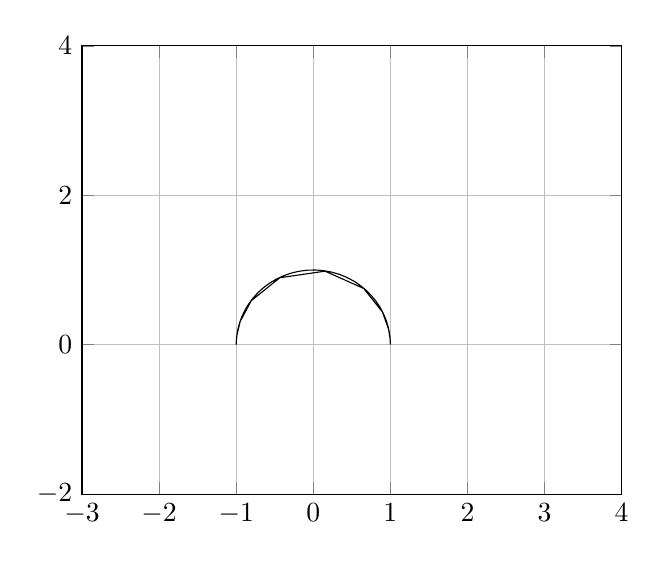
\begin{tikzpicture}
  \begin{axis}[
     xmin=-3,xmax=4,
     ymin=-2,ymax=4,
     grid=both,
    ]
    \addplot [domain=0:6.283,samples=50]({
      ( 2 * cos((x) r) * ((2)^(1/2) + sin((x) r)))/(3 + (2)^(3/2)*sin( (x) r))
    },{
      ((1 + (2)^(1/2)*sin((x) r))^2)/(3 + (2)^(3/2)*sin( (x) r))
    }); 
  \end{axis}
\end{tikzpicture}
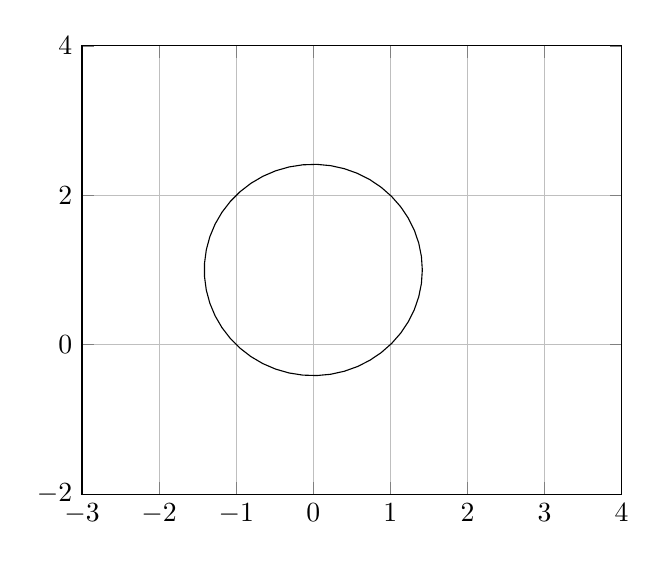
\begin{tikzpicture}
  \begin{axis}[
     xmin=-3,xmax=4,
     ymin=-2,ymax=4,
     grid=both,
    ]
    \addplot [domain=0:6.283,samples=50]({
      (2)^(1/2)*cos((x) r)
    },{
      1 + (2)^(1/2)*sin((x) r)
    }); 
  \end{axis}
\end{tikzpicture}


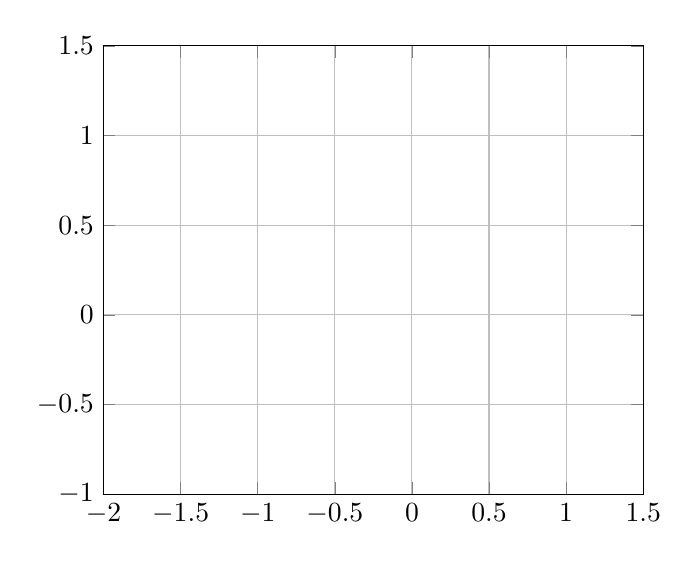
\begin{tikzpicture}
  \begin{axis}[
     xmin=-2,xmax=1.5,
     ymin=-1,ymax=1.5,
     grid=both,
    ]
    \airfoil{2}{pi/3}
  \end{axis}
\end{tikzpicture}
